\section{Advanced Tasks: Diarization \& Emotion Recognition}

\begin{frame}{}
    \LARGE \textbf{Advanced Tasks: Diarization \& Emotion Recognition}
\end{frame}

% --- Speaker Diarization Frame 1 ---
\begin{frame}[allowframebreaks]{Speaker Diarization}
    \begin{itemize}
        \item \textbf{Goal:} Identify "who spoke when" in audio streams
        \item \textbf{Applications:}
            \begin{itemize}
                \item Meeting transcription
                \item Podcast analysis
                \item Call center monitoring
            \end{itemize}
        \item \textbf{Pipeline:}
            \begin{enumerate}
                \item \textbf{Segmentation:} Detect speaker change points
                \item \textbf{Embedding:} Extract speaker features
                \item \textbf{Clustering:} Group segments by speaker
            \end{enumerate}
    \end{itemize}
    \begin{center}
        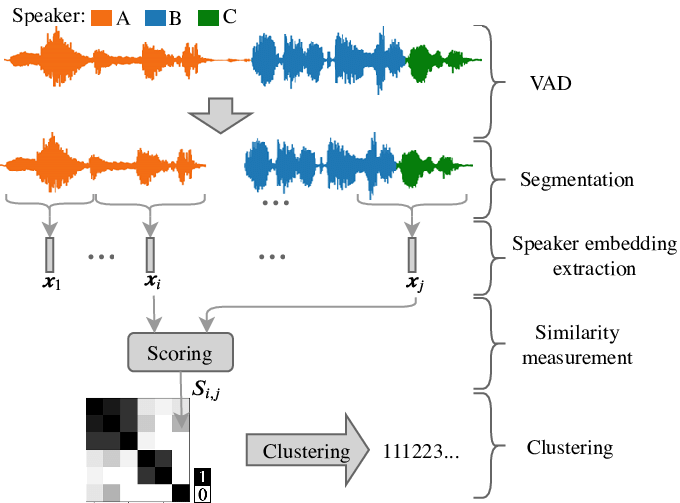
\includegraphics[width=\textwidth,height=0.9\textheight,keepaspectratio]{images/audio-nlp/diarization_pipeline.png}
    \end{center}
\end{frame}

% --- Speaker Diarization Frame 2 ---
\begin{frame}[allowframebreaks]{Speaker Diarization Tools}
    \begin{itemize}
        \item \textbf{Popular Tool:} \texttt{pyannote-audio}
        \item \textbf{Features:}
            \begin{itemize}
                \item Pre-trained diarization models
                \item Easy integration with Python
                \item Supports custom pipelines
            \end{itemize}
    \end{itemize}
    \begin{center}
        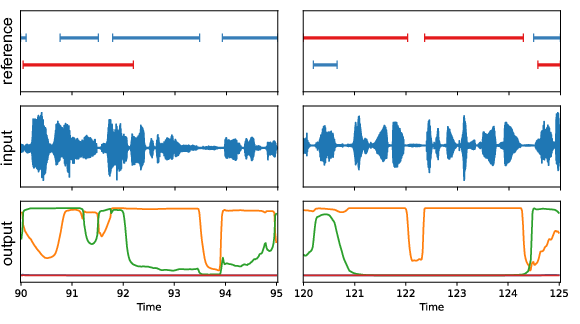
\includegraphics[width=\textwidth,height=0.9\textheight,keepaspectratio]{images/audio-nlp/pyannote_output.png}
    \end{center}
\end{frame}

% --- Emotion Recognition Frame 1 ---
\begin{frame}[allowframebreaks]{Emotion Recognition}
    \begin{itemize}
        \item \textbf{Goal:} Detect emotions from speech signals
        \item \textbf{Applications:}
            \begin{itemize}
                \item Human-computer interaction
                \item Mental health monitoring
                \item Customer service analytics
            \end{itemize}
        \item \textbf{Datasets:} IEMOCAP, YouTube, arXiv, PLOS
    \end{itemize}
    \begin{center}
        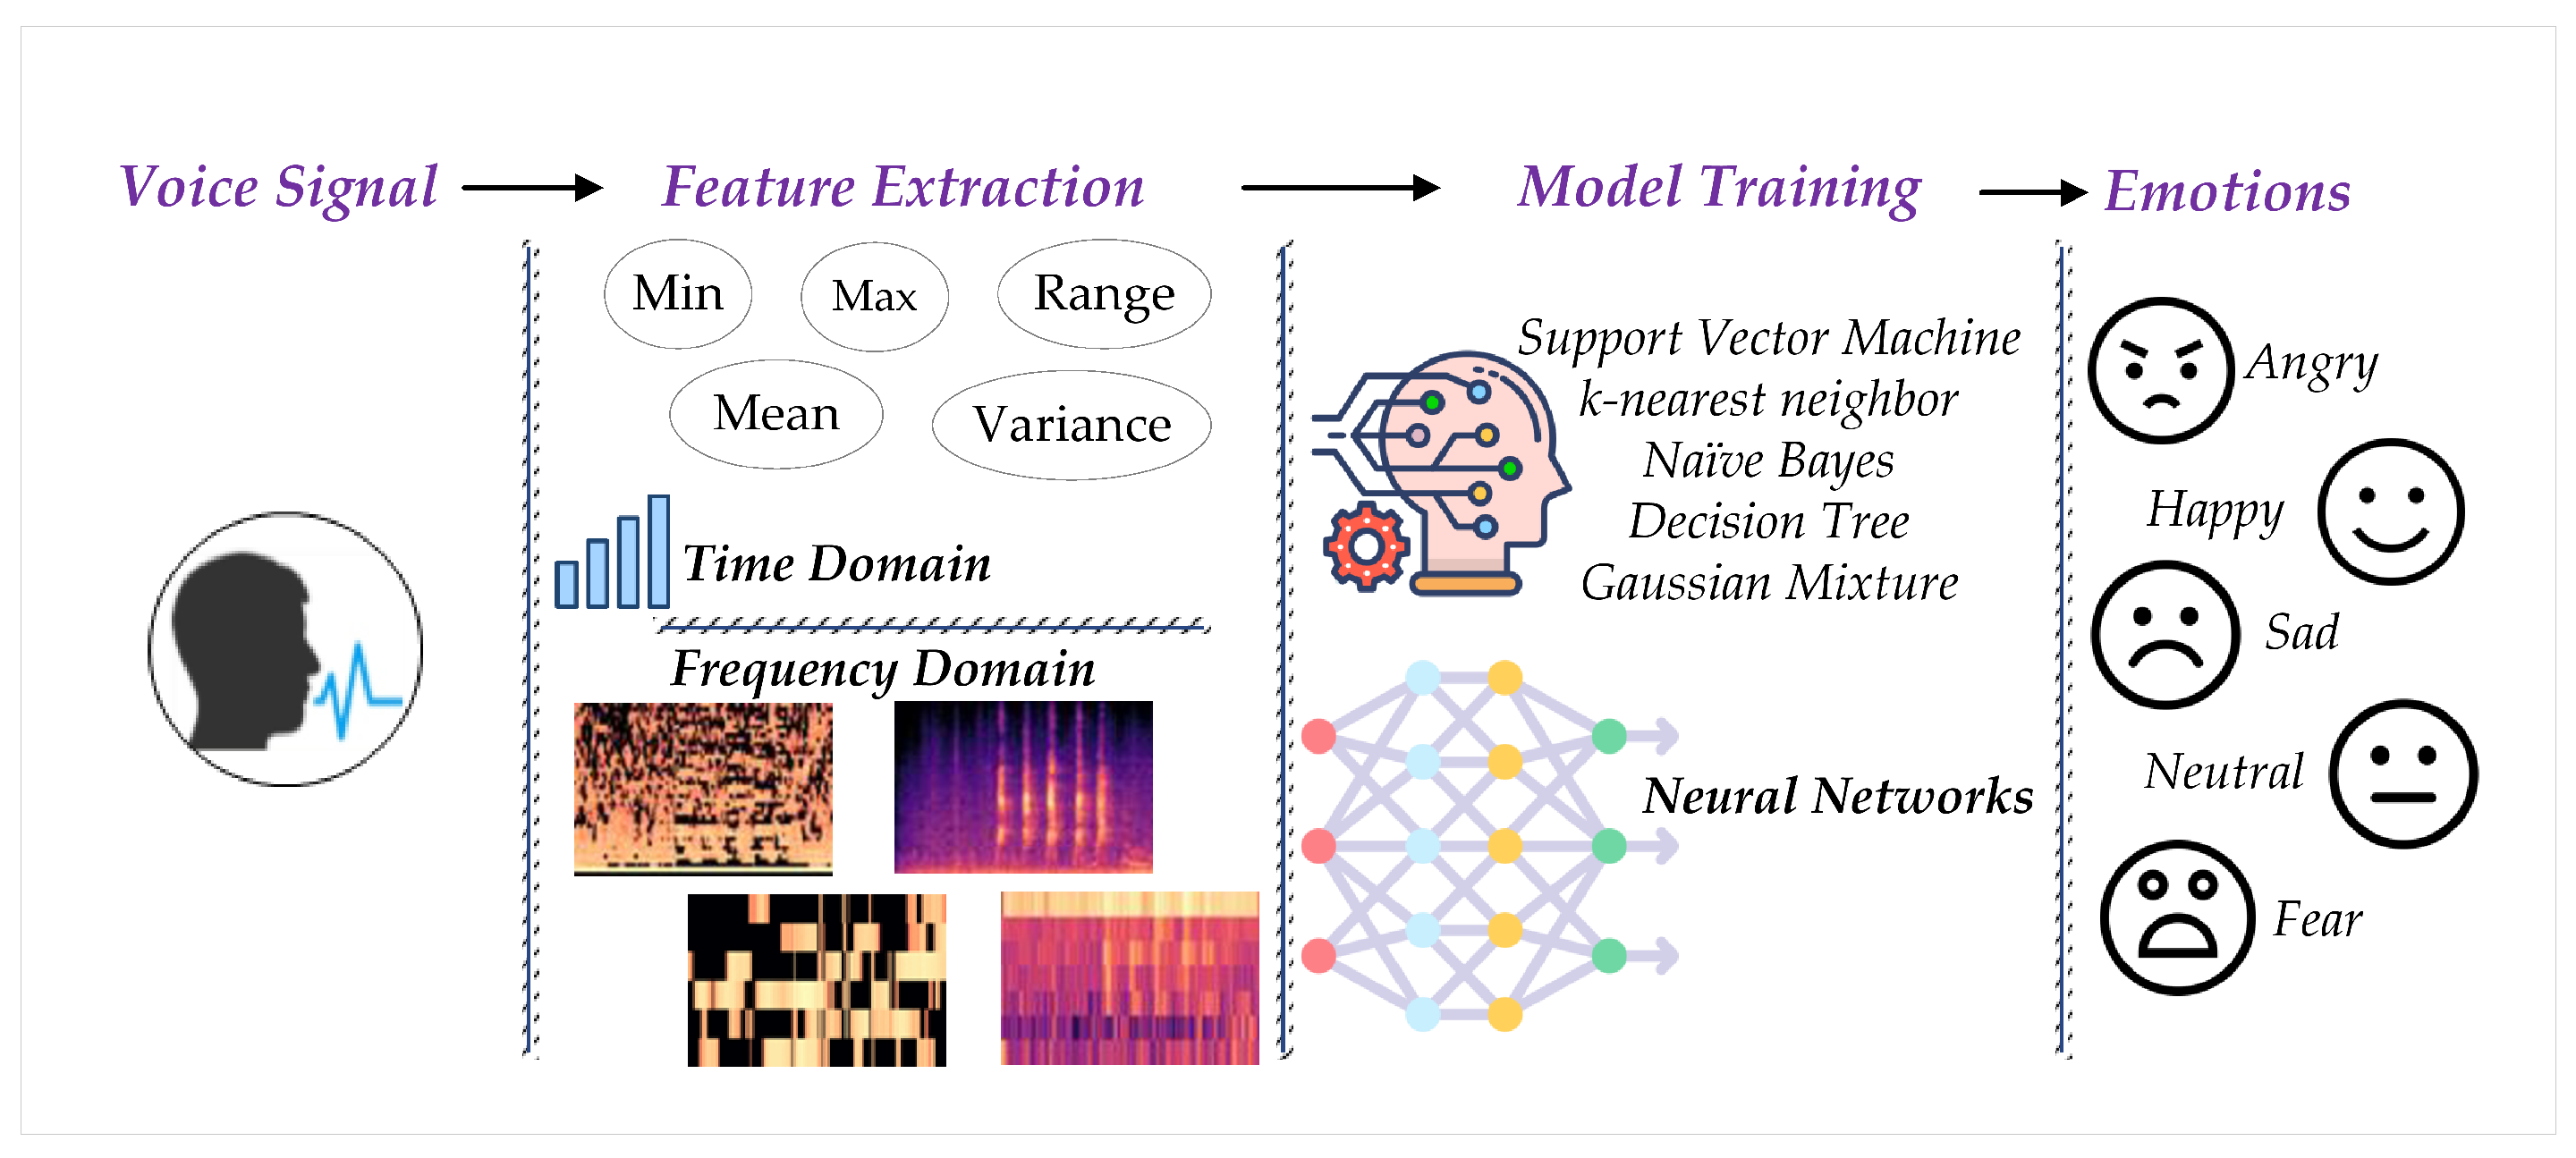
\includegraphics[width=\textwidth]{images/audio-nlp/emotion_classes.png}
    \end{center}
\end{frame}

% --- Emotion Recognition Frame 2 ---
\begin{frame}{Emotion Recognition: Models}
    \begin{itemize}
        \item \textbf{Wav2Vec 2.0:}
            \begin{itemize}
                \item Self-supervised speech representation
                \item Robust to noise and speaker variation
            \end{itemize}
        \item \textbf{Neural CDEs:}
            \begin{itemize}
                \item Continuous-time neural networks
                \item Capture temporal dynamics in speech
            \end{itemize}
        \item \textbf{Performance:}
            \begin{itemize}
                \item Achieves $\sim$70\% accuracy on IEMOCAP
            \end{itemize}
    \end{itemize}
    \begin{equation*}
        \text{Accuracy} = \frac{\text{Correct Predictions}}{\text{Total Samples}}
    \end{equation*}
\end{frame}

% --- Audio-Visual Speech Frame ---
\begin{frame}{Audio-Visual Speech Recognition (LipNet)}
    \begin{itemize}
        \item \textbf{LipNet:}
            \begin{itemize}
                \item Integrates lip movement and audio
                \item Robust speech decoding in noisy environments
            \end{itemize}
        \item \textbf{Benefits:}
            \begin{itemize}
                \item Improved accuracy
                \item Handles missing or corrupted audio
            \end{itemize}
    \end{itemize}
    \begin{center}
        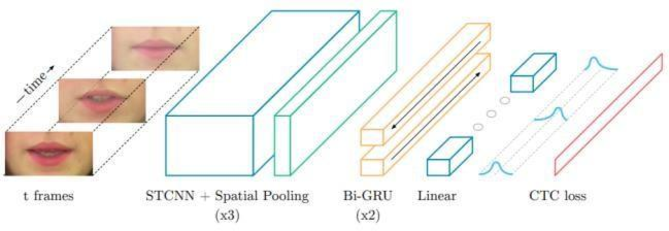
\includegraphics[width=0.9\textwidth]{images/audio-nlp/lipnet_architecture.png}
    \end{center}
\end{frame}